\documentclass[14pt,sans]{beamer}
\usepackage[utf8]{inputenc}
\usepackage[T1]{fontenc}
\usepackage{url}
\usepackage{hyperref}
\usepackage{graphicx}
\usepackage{listings}
\usepackage{pslatex}
\usepackage{beamerthemesplit}
\usepackage{courier}
\usepackage[german,english]{babel}
\usepackage{longtable}

\newcommand{\arrow}{\ensuremath{\rightarrow}\ }
\newcommand{\botharrow}{\ensuremath{\leftrightarrow}\ }
\newcommand{\us}{\ensuremath{\mu}s}

\newcommand{\task}[1]{\frqq #1\flqq}
\newcommand{\resource}[1]{\frqq #1\flqq}
\newcommand{\state}[1]{\emph{#1}}
\newcommand{\software}[1]{\emph{#1}}
\newcommand{\syscall}[1]{\texttt{#1}}
\newcommand{\hook}[1]{\texttt{#1}}
\newcommand{\codebig}[1]{\texttt{#1}}
\newcommand{\code}[1]{\small\texttt{#1}\normalsize}
\newcommand{\hlcode}[1]{\lstinline[language=c,inputencoding=latin1,basicstyle=\footnotesize\ttfamily,tabsize=4,breaklines=true,numberstyle=\tiny\sffamily,emph={TaskType,StatusType,EventMaskType,PriorityType,asm,__asm__},emphstyle={\textbf},showspaces=false,showstringspaces=false,numberblanklines=false]!#1!}
\newcommand{\file}[1]{\texttt{#1}}
\newcommand{\command}[1]{\texttt{#1}}
\newcommand{\jhook}[1]{\texttt{#1}}							% Do I need this?
\newcommand{\jdefine}[1]{\texttt{#1}}
\newcommand{\javaclass}[1]{\texttt{#1}}


% Multirow commands
\newcommand{\mrstart}[1]{\begin{minipage}[t]{#1}}
\newcommand{\mrend}{\vspace{0.15cm}\end{minipage}}

\useframetitletemplate{
	\renewcommand{\arraystretch}{0.5}
	\begin{structureenv}
		\tiny \ \\
		\Large
		\begin{tabular}{p{10cm}r}
			\insertframetitle & \small \insertframenumber/\inserttotalframenumber\\
		\end{tabular}
		\begin{tabular}{lp{10cm}}
			\small \ \ \ \  & \small \insertframesubtitle\\
		\end{tabular}
	\end{structureenv}
}

\beamersetleftmargin{1cm}
\beamersetrightmargin{1cm}

\title{Implementation of a User-Level-Firewall in Linux}
\author{Johannes Bauer, Severin Strobl}
\institute{Department of Computer Science 4}
\date{22nd of February 2008}

\begin{document}
\sffamily

\frame{\titlepage}

\section{Basics}
\frame{
	\frametitle{What does it do?}
	\begin{itemize}
		\item Why do we need it? What is this all about?
		\item Integration into LSM (Linux Security Modules)
		\item Kernel Level Interaction
		\item User Space interaction
	\end{itemize}
}

\section{Overview}
\subsection{Architecture}
\frame{
	\begin{center}
		\includegraphics[height=7cm]{figs/S_architecture_0}
	\end{center}
}

\frame{
	\begin{center}
		\includegraphics[height=7cm]{figs/S_architecture_1}
	\end{center}
}

\frame{
	\begin{center}
		\includegraphics[height=7cm]{figs/S_architecture_2}
	\end{center}
}

\frame{
	\begin{center}
		\includegraphics[height=7cm]{figs/S_architecture_3}
	\end{center}
}

\frame{
	\begin{center}
		\includegraphics[height=7cm]{figs/S_architecture_4}
	\end{center}
}

\frame{
	\begin{center}
		\includegraphics[height=7cm]{figs/S_architecture_5}
	\end{center}
}


\section{Kernel Level}
\subsection{Basic Interaction}
\frame{
	\begin{center}
		\includegraphics[width=\textwidth]{figs/J_01_Userspace_Kernelspace}
	\end{center}
}

\frame{
	\begin{center}
		\includegraphics[width=\textwidth]{figs/J_02_Userspace_Kernelspace_Simple}
	\end{center}
}

\frame{
	\begin{center}
		\includegraphics[width=\textwidth]{figs/J_03_Ringpuffer}
	\end{center}
}

\subsection{poll()}
\frame{
	\begin{center}
		\includegraphics[width=\textwidth]{figs/J_04_Progress}
	\end{center}
}

\frame{
	\begin{center}
		\includegraphics[width=\textwidth]{figs/J_05_Progress_Insert}
	\end{center}
}

\frame{
	\begin{center}
		\includegraphics[width=\textwidth]{figs/J_06_Progress_Wakeup}
	\end{center}
}

\frame{
	\begin{center}
		\includegraphics[width=\textwidth]{figs/J_07_Progress_Completion}
	\end{center}
}

\frame{
	\begin{center}
		\includegraphics[width=\textwidth]{figs/J_08_Progress_PollEnd}
	\end{center}
}

\subsection{read() and write()}
\frame{
	\begin{center}
		\includegraphics[width=\textwidth]{figs/J_09_Progress_Read}
	\end{center}
}

\frame{
	\begin{center}
		\includegraphics[width=\textwidth]{figs/J_10_Progress_Write}
	\end{center}
}

\frame{
	\begin{center}
		\includegraphics[width=\textwidth]{figs/J_11_Progress_Finished}
	\end{center}
}

\section{User Space Daemon}
\subsection{Main Loop}
\frame{
	\begin{center}
		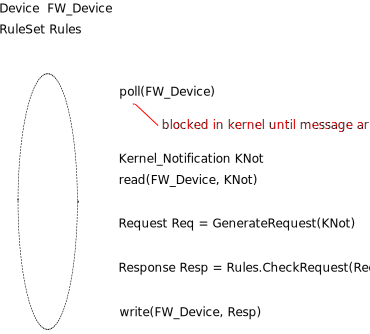
\includegraphics[height=6cm]{figs/S_acherond}
	\end{center}
}

\subsection{Rules}
\frame{
	\begin{center}
		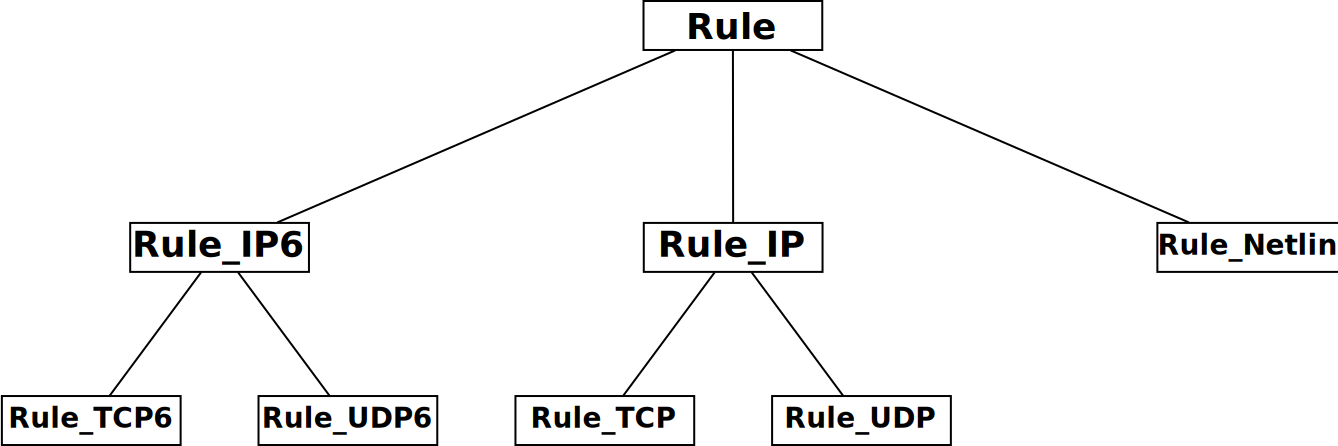
\includegraphics[width=\textwidth]{figs/S_Rules}
	\end{center}
}

\frame{
	\begin{center}
		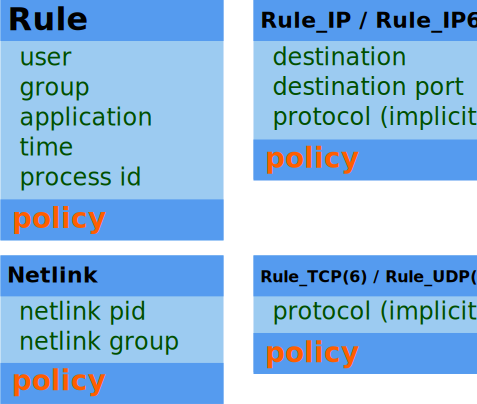
\includegraphics[height=6cm]{figs/S_RuleMatching}
	\end{center}
}

\frame{
	\frametitle{Are there any more...}
	\begin{center}
		\Huge Questions?
	\end{center}
}

\end{document}

